\subsection{Shorter does not imply faster}
\label{sec:shorternotfaster}
We will shortly investigate, which properties of paths are desirable. Firstly a shorter path does not necessarily imply a faster path for electric vehicles. This is partly due to the fact that electric vehicles use polynomially more energy as their speed increases, but also due to the fact that charge times on charging stations varies a lot. Driving a longer path with a fast charging station, can therefore turn out to be a faster choice than driving a shorter path with a slow charging station. This is illustrated in Figure \ref{fig:simpleroad-network}. In the example, we assume our car has a battery capacity of 100 $\si{\kWh}$ and a consumption rate of 0,4 $\si{\kWh\per\km}$ at the speed of 100 $\si{\km\per\hour}$.

Path 1 consists of two edges with distance: $ 250 \si{\km}$ and speed limit: $100 \si{\km\per\hour}$
and a charging station with a charge speed of 200 $\si{\kW}$. Path 2 consists of two edges with distance: $200 \si{\km}$ and speed limit: $100 \si{\km\hour}$ and a charging station with a charge speed of $30\si{\kW}$. The current battery capacity of the vehicle is noted at each vertex in parenthesis. The total time of each path:
				
\textbf{Path 1:} $\frac{250\si{km} + 250\si{km}}{100\si{\km\per\hour}} + \frac{100\si{\kWh}}{200\si{\kW}} = 5.5\si{\hour}$

\textbf{Path 2:} $\frac{200\si{km} + 200\si{km}}{100 \si{\km\per\hour}} + \frac{60\si{\kWh}}{30\si{\kW}} = 6\si{\hour}$


\begin{figure}
\centering
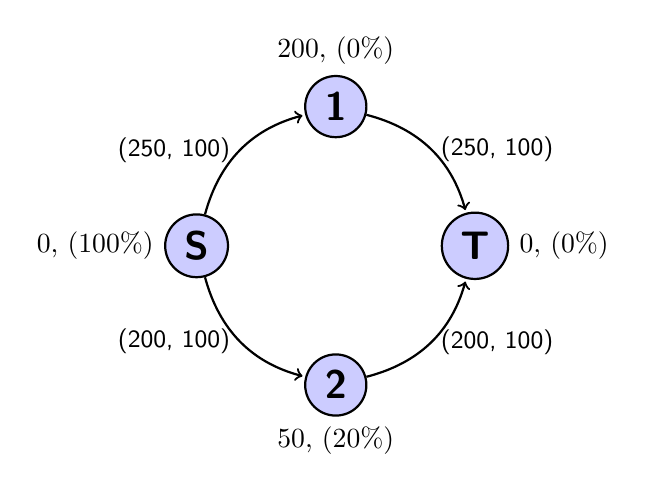
\begin{tikzpicture}[
->,->, shorten >=1pt,scale=0.1,node distance=2.5cm,thick,
main node/.style={circle,fill=blue!20,draw,font=\sffamily\Large\bfseries}]
%1
  \node[main node] (1) {1};
  \node[above] at (1.north) {200, (0\%)};
%2 
 \node[main node] (2) [below left of=1] {S};
  \node[left] at (2.west) {0, (100\%)};
%3 
 \node[main node] (3) [below right of=2] {2};
  \node[below] at (3.south) {50, (20\%)};
%4 
 \node[main node] (4) [below right of=1] {T};
  \node[right] at (4.east) {0, (0\%)};
%paths
  \path[every node/.style={font=\sffamily\small}]
    (1)
      edge [bend left] node[right] {(250, 100)} (4)
    (2) edge [bend right] node[left] {(200, 100)} (3)
          edge [bend left] node[left] {(250, 100)} (1)
    (3) edge [bend right] node[right] {(200, 100)} (4)
    (4) ;
\end{tikzpicture}
\label{fig:simpleroad-network}
\caption{A simple road network with starting point s and end point t. The charge rates on the road network dictates that the longer path is in fact the fastest}
\end{figure}